\chapter{Methods and Results}
% Patchy particle scheme for hydrophilic polymeric networks

Now that the theoretical framework was covered, lets delve into the numerical tools that will help to find relations between the polymeric network and the mechanical response. 
First, the patchy particle scheme for simulating PNIPAM cross-linked networks is presented, detailing the numerical simulation protocol.
Also an introduction to the LAMMPS software and how it was used to simulate this system is covered.
To finished the chapter, the numerical results are analyzed.

\section{Simulation protocol}

One of the microgels that has been the focus of significant research is the type that is based on PNIPAM cross-linked networks.
In the article \textit{In silico Synthesis of Microgel Particles}\citep{gnanSilicoSynthesisMicrogel2017}, the authors present a flexible numerical protocol capable of designing individual microgel particles based on PNIPAM crosslinked networks. 
This protocol can generate particles with properties comparable to the experimental ones.
In this project, we employ a similar protocol to explore its versatility and identify a numerical tool that can facilitate connections between network configuration and mechanical response.

The primary focus is on creating networks without spherical confinement and without mimicking the swelling behavior of PINIPAM microgels with temperature.
As a result, the central technique involves using a binary mixture of patchy particles to create a disordered polymeric network structure, which is then deformed using shear forces.
The primary benefit of this protocol is that previous numerical efforts in microgel modeling have predominantly concentrated on unrealistic networks consisting of chains of equivalent length, frequently establishing cross-linked connections on crystalline lattice regions or where closed polymer networks are assembled by directly integrating randomly dispersed cross-linkers with polymer chains.

\subsection{Patchy particles representation}

A patchy particle\citep{bianchiPhaseDiagramPatchy2006,bianchiTheoreticalNumericalStudy2008} can be defined as a sphere with radius $r$ containing $n$ spheres of radius $l<r$ on its surface.
The smaller spheres are typically referred to as ``patches,'' and the number of patches is often referred to as ``functionality''.
The center of the patches can be placed on the surface of the central particle. 
However, it can also be modified to be at a point inside the enclosed volume of the main particle.

The use of patchy particles as monomers and crosslinkers is a highly effective method since it allows for the integration of Langevin dynamics' infinitesimal representation with a particle with volume and functionality.
The functionality is important because it allows for the representation of the monomer and cross-linker molecules that can form a polymeric network.
However, it is important to note that the monomers and interaction sites are considered to be spherical.

To define the volume of the particle, a repulsive pairwise interaction is defined between the central particles.
Meanwhile, the formation of the polymeric network is encouraged by a pairwise interaction between patches.
Because this model is designed to simulate the final network, not the synthesis process, the pairwise interaction between central particles and patches is not defined.
%In contrast, the softness explained by particle interactions is characterized by the form of the repulsive pair potential between two particles.
Finally, the particle volume fraction contributes to the ability of the particles to deform or compress, in contrast to hard spheres\citep{vlassopoulosTunableRheologyDense2014}.\footnote{The patchy particles are hard spheres, but the hydrogel network is a soft ``particle''.}

\subsection{Description of the system}

%\paragraph{Interaction potentials}
Let's start by describing the interaction potentials between patchy particles.
The interaction between the central particles is modeled using a Weeks-Chandler-Andersen repulsive potential.
\begin{gather}
    U_{WCA}(r_{i,j}) =\left\{ 
        \begin{array}{ll}
            4\epsilon_{i,j}\left[\qty(\frac{\sigma}{r_{i,j}})^{12}-\qty(\frac{\sigma}{r_{i,j}})^6\right]+\epsilon_{i,j}, & r_{i,j}\in[0,2^{1/6}\sigma], \\
            0, & r_{i,j}>2^{1/6}\sigma
        \end{array}
\right.
    ,\label{eqn:CL-MO_interaction}
\end{gather}
where $r_{i,j}$ is the distance between the center of the central particles, $\sigma$ is the diameter of the particles and $\epsilon_{i,j}$ is the energy of the interacton.
On the other hand, the patch-patch interaction is modeled with an attractive potential,
\begin{gather}
    U_{\mathrm{patchy}}\qty(r_{\mu\upsilon}) = \left\{
        \begin{array}{ll}
            2\epsilon_{\mu\upsilon}\left(\frac{\sigma_p^4}{2 r_{\mu\upsilon}^4}-1\right)\exp\left[\frac{\sigma_p}{\qty(r_{\mu\upsilon}-r_{c})}+2\right], & r_{\mu\upsilon}\in\qty[0,r_c], \\
            0, & r_{\mu,\upsilon}>r_c,
        \end{array}
            \right.\label{eqn:patch-patch_interaction}
\end{gather}
where $r_{\mu\upsilon}$ is the distance between two patches, $\sigma_p$ is the diameter of the patches, $r_c$ is the cut distance of interaction set to $1.5\sigma_p$ and $\epsilon_{\mu,\upsilon}$ is the interaction energy between the patches.
%This potential can be interpreted as a reversible interaction.

In order to put in context the type of polymeric network that this potentials models, equation~\eqref{eqn:patch-patch_interaction} is compared with the FENE potential,
\begin{equation}
    U_{\mathrm{FENE}}(r) = -\frac{1}{2}KR_o^2\ln\left[1-\left(\frac{r}{R_o}\right)^2\right]+U_{WCA}(r),\label{eqn:FENEpot}
\end{equation}
where $R_o$ is the maximum extent of the bond and $K$ is the energy of the bond and has units of energy over area.
This potential it is used to represent covalent bonds between monomers in a polymers.

Figure~\ref{fig:patchpatchpot} compares the patch-patch interaction potential, the Lennard-Jones potential, and the FENE potential.
The Lennard-Jones and patch-patch potentials are qualitatively similar in that they both tend to zero after a certain cutoff distance.
In contrast, the FENE potential goes to infinity if the distance is too short or too wide.
This key distinction enables us to design the patch-patch interaction as a reversible interaction rather than the FENE, which is better suited to representing non-reversible interactions.
As a result, the computational methodology simulates a polymeric network with physical crosslinkers.

\begin{figure}[ht!]
    \centering
    \includegraphics[width=12cm]{figs/numerical/patchpatch.png}
    \caption{Comparisson between the potentials used in the simulation with standard potentials.
        Orange and green line are the potentials used in the simulation for the interaction between central particles and patches, respectively.
        While, the blue and red are the Lennard-Jones and FENE potentials, commonly used to represent interparticle interactions.
        All distances where modifed to match the patches particles for comparison reasons.
}\label{fig:patchpatchpot}
\end{figure}

The patch-patch interaction differs from the Lennard-Jones potential in that the minimum potential is horizontally translated, and the rate of change from the minimum to the cut distance is more apparent.
Equation~\eqref{eqn:patch-patch_interaction} represents a stronger interaction between the patches compared to a Lennard-Jones potential.

However, if the simulation for the polymeric network is simply performed using the Lennard-Jones and patch-patch potentials, the patches will form interactions of more than two patches, which is undesirable.
Hence, the interaction between patches is complemented by a three-body repulsive potential, defined in terms of~\eqref{eqn:patch-patch_interaction}, that provides an efficient bond-swapping mechanism, making it possible to easily equilibrate the system even at low temperatures, while at the same time retaining the single bond per patch condition\citep{sciortinoThreebodyPotentialSimulating2017}.
This interaction is given by:
\begin{gather}
    U_{\mathrm{swap}}(r_{l,m},r_{l,n}) = w\sum_{l,m,n}\epsilon_{m,n}U_3\qty(r_{l,m})U_3\qty(r_{l,n}),\quad r_{l,n}\in\qty[0,r_c],\label{eqn:swap_interaction}
\end{gather}
where
\begin{gather}
    U_{3}\qty(r) = \left\{
        \begin{array}{ll}
            1 & r\in\qty[0,r_{\min}], \\
            -U_{\mathrm{patchy}}\qty(r)/\epsilon_{m,n}, & r\in\qty[r_{\min},r_c]
        \end{array}
        \right.\label{eqn:swapmod_interaction}.
\end{gather}
The sum in~\eqref{eqn:swap_interaction} runs over all triples of bonded patches (patch $l$ bonded both with $m$ and $n$).
$r_{l,m}$ and $r_{l,n}$ are the distances between the reference patch and the other two patches.
The parameter $\epsilon_{m,n}$ is the energy of repulsion, and $w$ is used to tune the swapping ($w=1$) and non-swapping bonds ($w\gg1$). 
The cutoff distance $r_c$ is the same as in the potential of interaction between patches, meanwhile the minimum distance $r_{\min}$ is the distance at the minimum of~\eqref{eqn:patch-patch_interaction}, \textit{i.e.} $\epsilon_{m,n}\equiv\abs{U_{\mathrm{patchy}}(r_{\min})}$.

Figure~\ref{fig:swappot}\footnote{Be carefull with the sign interpretation and more detail about the different curves.} shows the patch-patch potential with the swap potential.
The patch-patch potential in the figure is the energy of the interaction between patch $i$ and patch $k$.
The swap potential is the energy between patch $i$ and patch $k$, leaving the distance between patch $i$ and patch $j$ fixed.
Taking into account this, when the patches $i$ and $j$ are at the potential well ($r_{ij}=\sigma$), the interaction between $i$ and $k$ is null.
When the distance between patches $i$ and $j$ are bigger than the potential well but smaller than the cutoff distance ($r_{\mathrm{cut}}>r_{ij}>\sigma$), the interaction between $i-k$ is mildly attractive.
Finally, when the patches $i-j$ are bigger than the cutoff distance ($r_{\mathrm{cut}}<r_{ij}$), the interaction between $i-k$ is repulsive.

\begin{figure}[ht!]
    \centering
    \includegraphics[width=12cm]{figs/numerical/swapPotential.png}
    \caption{Swap potential for patch-patch interaction to ensure single bond per patch condition.
        Blue line represents the patch-patch interaction potential.
        Orange, green and red lines represent the swap potential with a fix distance between patch $i$ with patch $j$ and a free patch $k$.
        When the patches $i$ and $j$ are at the potential well, the interaction between partches $i-k$ and $j-k$ is repulsive (orange line).
        However, when the distance between patches $i$ and $j$ starts to increase, the repulsive interaction with patch $k$ diminishes.
    }\label{fig:swappot}
\end{figure}

Before proceeding to the description of the parameters for the simulation, it is necessary to describe the interaction between the central particle and the patches.
The patches and the central particles are linked by harmonic potentials.
\begin{align}
    E_r &= K_r\qty(r-r_{o})^2, \\
    E_\theta &= K_\theta\qty(\theta-\theta_{o})^2.
\end{align}
Where $r_o$ and $\theta_o$ represent the equilibrium bond distance and angle.
Meanwhile, $K$ is equal to $K=k/2$, where $k$ is the energy of the bond.
This allows us to create patchy particles with patches fixed at a convenient position.

All of the above descriptions are summarized in figure~\ref{fig:interactionPatches}.
Orange central particles indicate patchy particles with valence \num{2}, while red central particles indicate patchy particles with valence \num{4}, as illustrated in panels a and b.
On panels c and d, we can see the swap dynamic enabled by the three-body potential.
On panel C, a patchy particle approaches a pair of bonded patches.
Because of the swap potential, instead of forming a bond between the three patches, the interaction can shift to form a bond with the incoming particle.

\begin{figure}[ht!]
    \centering
    \includegraphics[width=8cm]{figs/numerical/interactionPatches.png}
    \caption{Interaction between patchy particles}\label{fig:interactionPatches}
\end{figure}

%\paragraph{Polymeric network parameters}
Let us now move on to the simulation's parameters.
Each system had a fixed number of patchy particles $N_p$, packing fraction $\phi$, and cross-link concentration $c$.
Based on these characteristics, we calculate the box's volume as well as the number of patchy particles of functionality 2 (PB) and functionality 4 (PA).

Due to limitations related to time and computing resources, the total number of particles is set to be $N_p=\num{8000}$.
This is a lower number of particles when compared with other simulations~\citep{gnanSilicoSynthesisMicrogel2017}.
Therefore, in order to compensate, we take the mean of five experiments.
In addition, the timestep was set to \num{0.001}, as a rule of thumb.
This allow us to obtain good average observables.
Finally, the values of $K_r$ and $K_\theta$ are set to \num{100} to create a strong bond and prevent stretching of monomers (patchy particles B) and crosslinkers (patchy particles A).
The value of $r_o$ is set to \num{0.45}.
The value of $\theta_o$ is set to \SI{180}{\degree} for PB particles and \SI{109.4712}{\degree} for PA particles.

Once the parameters for the synthesis were set, the volume of the box was calculated by determining the volume of the patchy particles A and B and then scaling those values by the number of particles and the desired packing fraction.
\begin{align*}
    V_{\mathrm{box}} &= \frac{N_{\mathrm{patchyA}}V_{\mathrm{patchyA}}+N_{\mathrm{patchyB}}V_{\mathrm{patchyB}}}{\phi}
\end{align*}
The number of patchy particles of type A is computed as $N_{\mathrm{patchyA}} = c N_p$, and the number of patchy particles of type B as $N_{\mathrm{patchyB}}= N_p - N_{\mathrm{patchyA}}= N_p(1 - c )$.
Finally, the temperature was set to be constant through all the assembly process, $T=\num{0.05}$ in Lennard-Jones units; meanwhile, the damp parameter was set to $\mathrm{damp}=\num{0.5}$.
It is very important to note that the damp controls the viscous response caused by the interaction between the thermal bath and the particles, which symbolizes the interaction of water molecules with the polymer network. The radius of the central particle is set to $0.5$ ($\sigma=1$) and the radius of the patches at $0.2$ ($\sigma_p=0.4$).

The energy of interaction between central particles is 1 $\epsilon_{i,j}=1$.
In contrast, the energy of interaction between patches is defined as follows:
The interaction of patchy particles B is set to 1 ($\epsilon_{\mu,\upsilon}=1$), whereas the interaction between patchy particles A is set to \num{0} ($\epsilon_{\mu,\upsilon}=0$), and the interaction between patches of patchy particles A with patchy particles B is set to \num{1} ($\epsilon_{\mu,\upsilon}=1$).
This is to allow only crosslinker-monomer and monomer-monomer bonding.

%\paragraph{Deformation protocol}
Once the assembly simulation of the patchy particle network was done, we performed a shear deformation to the resulting network.
We select the shear deformation because shear forces dominate biological environments where hydrogels are typically deployed. 
Also, shear testing provides a more uniform stress field throughout the hydrogel sample compared to tensile testing. 
In rheological measurements using parallel plate or cone-and-plate geometries, the applied shear stress is distributed evenly across the sample, eliminating edge effects and stress concentrations that plague tensile testing.
Furthermore, shear rheometry excels at characterizing the complex viscoelastic properties that define hydrogel functionality.
Many hydrogels exhibit shear-thinning behavior that is critical for applications like injection and 3D bioprinting. 
The shear deformation was done at a constant shear rate in the $xy$ plane.

The shear rates were in the \num{d-3} order of magnitude, and the final strain was \num{15} units.
This is to characterize the mechanical response and to deform beyond the plastic deformation limit.
Also, the variation of the shear rate was performed to see the viscoelastic response of the material.
The temperature and dampness parameters were set to be the same as in the assembly process.

\subsection{LAMMPS implementation}

As said before, LAMMPS software is used to solve the Langevin equation in a many-particle system.
However, it is useful to explain how the simulation is defined in this software.
In this regard, in the next paragraphs, it briefly discusses the $\mathrm{damp}$ parameter, the implementation of the swap potential~\eqref{eqn:swapmod_interaction}, the shear deformation, and the calculation of the stress tensor.

%\paragraph{damp}
Comparin equation~\eqref{eqn:MolDylammps1} with equation~\eqref{eqn:MolDylammps2}, the viscosity parameter $\gamma$ of the Langevin equation~\eqref{eqn:BrownianDyn1} does not appear; instead, the $\mathrm{damp}$ parameter appears.
This parameter is specified in time units and determines how rapidly the temperature is relaxed so that it can be more easily used as a thermostat\citep{LAMMPS}.
That is, if damp is set to \num{100}, the temperature will relax in a timespan of roughly \num{100} time units.
By making dimensional analysis, the damp factor can be thought of as inversely related to the viscosity of the solvent.
This tells us that a small damp represents a high-viscosity solvent and vice versa.
Therefore, since the damp is set to \num{0.1}, the polymeric network is in a high-viscosity solvent.
In addition it is important to mention that all the simulations are done with Lennard Jones units.

%\paragraph{Three-body potential}
Moving towards the implementation of the swap potential.
The \verb|threebody/table| pair style command is used to implement generic tabulated three-body interactions.
However, in LAMMPS, the tabulation is done on a three-dimensional plane of the two distances $r_{ij}$ and $r_{ik}$ with the angle $\theta_{ijk}$, where the forces on all three particles $I$, $J$, and $K$ lie within the plane defined by the three inter-particle distance vectors $\vec{r}_{IJ}$, $\vec{r}_{IK}$, and $\vec{r}_{JK}$\citep{LAMMPS}.
Allowing the following property to project the forces onto the inter-particle distance vectors,
\begin{equation}
    \begin{pmatrix}\vec{f}_i \\ \vec{f}_j \\ \vec{f}_k\end{pmatrix}
    =
    \begin{pmatrix}f_{i1} & f_{i2} & 0 \\ f_{j1} & 0 & f_{j2} \\ 0 & f_{k1} & f_{k2} \end{pmatrix}
    \begin{pmatrix}\vec{r}_{ij} \\ \vec{r}_{ik} \\ \vec{r}_{jk}\end{pmatrix}.
\end{equation}
And due to symmetry interactions, $f_{i1}=-f_{j1}$, $f_{i2}=-f_{k1}$, and $f_{j2}=-f_{k2}$.

Therefore, to have a correct tabulation, it is necessary to project the force into the inter-particle plane.
Recalling that the force is equivalent to $-\nabla U(r)$ and the potential has only radial dependence, the force can be expressed as
\begin{gather}
    \vec{f}_n = -\pdv{U_{\mathrm{swap}}(r_m,r_l)}{r}\hat{e}_r,
\end{gather}
where $n$ represent the particle $i$, $j$ or $k$, while $m$ and $l$ are place holders for distances $ij$, $ik$ and $jk$.
Hence, 
\begin{align}
    \vec{f_{i}} &= -\pdv{U_{\mathrm{swap}}(r_{ij},r_{ik})}{r}\hat{e}_r\label{eqn:3body1}, \\
    \vec{f_{j}} &= -\pdv{U_{\mathrm{swap}}(r_{ji},r_{jk})}{r}\hat{e}_r\label{eqn:3body2}, \\
    \vec{f_{k}} &= -\pdv{U_{\mathrm{swap}}(r_{ki},r_{kj})}{r}\hat{e}_r\label{eqn:3body3}.
\end{align}
The projection of the force into the plane is computed via the dot product between $\hat{e}_r$ and the basis that represents the plane. 
Which can be defined by the following 2-dimensional basis, $\hat{e}_1=\qty[1,0] $ and $\hat{e}_2=\qty[\cos\theta,\sin\theta] $, and $\theta$ is the angle between distances $\vec{r}_{ij}$ and $\vec{r}_{ik}$ since the software defines the plane using the distances between the particles.
With this we can compute the following projections:
\begin{align}
    \hat{e}_r \cdot \hat{e}_1 &= 1\\
    \hat{e}_r \cdot \hat{e}_2 &= \cos\theta. 
\end{align}
Also, the following vector can be defined as $\hat{e}_3 = \hat{e}_1 - \hat{e}_2 = \qty[1-\cos\theta,-\sin\theta]$ to represent the $j-k$ distance, and the projection will be
\begin{align}
    \hat{e}_r \cdot \hat{e}_3 &= 1-\cos\theta.
\end{align}

With these projections the forces can be expressed in~\eqref{eqn:3body1},~\eqref{eqn:3body2}, and~\eqref{eqn:3body3} as follows:
\begin{align}
    f_{i1} &= -\pdv{U_{\mathrm{swap}}(r_{ij},r_{ik})}{r}\label{eqn:3body4a}, \\
    f_{i2} &= -\pdv{U_{\mathrm{swap}}(r_{ij},r_{ik})}{r}\cos\theta\label{eqn:3body4b}, \\
    f_{j2} &= -\pdv{U_{\mathrm{swap}}(r_{ji},r_{jk})}{r}\qty(1-\cos\theta)\label{eqn:3body5}.
\end{align}
And due to the symmetry relations, the potential can be tabulated into the LAMMPS software to introduce the one-bond-per-patch condition and mitigate numerical instability during shear deformation.

The \verb|fix deform| command simulates a shear deformation on the $xy$ plane.
It uses the engineering deformation rate (\verb|erate| style) to adjust the box's dimension at a ``constant engineering strain rate''.
The length of the box, L, will be modified over time,
\begin{gather}
    L(t) = L_o\qty(1 + \mathrm{erate}~dt),
\end{gather}
where $L_o$ is the original box length and $\mathrm{erate}$ is the shear rate in units of $1/\mathrm{time}$\citep{LAMMPS}.
This deformation is applied in the $xy$ plane, and the change in length is along the $x$ direction.
This set of parameters ensures that the volume does not change during the deformation\citep{LAMMPS}.
In addition to the \verb|erate| style, the \verb|remap| keyword was set to \verb|x| to remap particle positions without affecting their velocities\citep{LAMMPS}.
Setting remap to x causes the atoms to deform using an affine transformation that is identical to the box deformation.  It is important to note that, while the atoms are effectively ``moving'' with the box over time, this is due to the remapping rather than their velocity, which tracks the box's change.
Finally, the \verb|flip| keyword is used to flip the box when the tilt factors exceed half the distance of the parallel box length to avoid computational inefficiency and errors\citep{LAMMPS}.

%\paragraph{fix stress} 
This section concludes with an explanation of how LAMMPS computes the stress tensor.
The \verb|compute stress/atom| calculates the stress tensor for an atom $I$ using the equation \citep{thompsonGeneralFormulationPressure2009,LAMMPS},
\begin{gather}
    S_{ab} = -v_a v_b - W_{ab}\label{eqn:stressLAMMPS},
\end{gather}
where $a$ and $b$ represent the spatial coordinates $x$, $y$ and $z$, and $W_{ab}$ is the virial contribution given by
\begin{multline}
    W_{ab} = \frac{1}{2}\sum_{n=1}^{N_p}\qty(r_{1a} F_{1b} + r_{2a} F_{2b})
            +\frac{1}{2}\sum_{n=1}^{N_b}\qty(r_{1a} F_{1b} + r_{2a} F_{2b}) \\
            +\frac{1}{3}\sum_{n=1}^{N_a}\qty(r_{1a} F_{1b} + r_{2a} F_{2b} + r_{3a} F_{3b})
            +\frac{1}{4}\sum_{n=1}^{N_d}\qty(r_{1a} F_{1b} + r_{2a} F_{2b} + r_{3a} F_{3b} + r_{4a} F_{4b}) \\
            +\frac{1}{4}\sum_{n=1}^{N_i}\qty(r_{1a} F_{1b} + r_{2a} F_{2b} + r_{3a} F_{3b} + r_{4a} F_{4b}) 
            +\sum_{n=1}^{N_f}r_{ia} F_{ib}.
\end{multline}
The first term accounts for pairwise interactions, the second for bond contributions, and the third, fourth, and fifth for angle-based interactions.
Since we only declare pairwise interactions and bond and angle interactions, the virial contribution simplifies to
\begin{multline}
    W_{ab} = \frac{1}{2}\sum_{n=1}^{N_p}\qty(r_{1a} F_{1b} + r_{2a} F_{2b})
            +\frac{1}{2}\sum_{n=1}^{N_b}\qty(r_{1a} F_{1b} + r_{2a} F_{2b}) \\
            +\frac{1}{3}\sum_{n=1}^{N_a}\qty(r_{1a} F_{1b} + r_{2a} F_{2b} + r_{3a} F_{3b})\label{eqn:virialLAMMPS}.
\end{multline}

Substituting the virial term~\eqref{eqn:virialLAMMPS} into the per-particle stress tensor~\eqref{eqn:stressLAMMPS} yields a similar expression for the previously derived stress~\eqref{eqn:DerVirTen23}.
The stress tensor in equation~\eqref{eqn:DerVirTen23} is a temporal and spatial average, whereas the stress tensor in~\eqref{eqn:stressLAMMPS} is defined per particle.
As a result, in order to study the mechanical response of the Cauchy stress tensor, a suitable time average, followed by a spatial average of the per-particle stress tensor along the patchy particle network, including the patches, is required.

\subsection{Assembly simulation and Shear deformation}

Now let's explain the simulation protocols for the assembly of the polymeric network and the applied deformation.
The assembly process starts by introducing the $N_p$ patchy particles at random positions in a box with lengths that match the desired packing fraction.
Then, the temperature is linearly increased from \num{0} to \num{0.05} in \num{500000} time steps to prevent numerical instability.
After that, the temperature was held constant until the total energy of the system stabilized to a minimum.
This process was performed by varying the number of time steps until it was found that the patchy particle network percolated and the energy of the system didn't increase.
The number of time steps that these conditions were met is \num{8d6} time steps after the previous \num{5d5}.

After the assembly protocol was completed, the final configuration was saved to a file before applying shear deformation.
The patchy particle network was then subjected to a series of five deformations with matching shear rates.
For each shear deformation simulation, the system energy, stress tensor components, temperature, and phase space configurations were saved.
Following 5 sets of deformation with the same shear rate, a new set of deformations was performed with a different shear rate, beginning with the same initial configuration as the previous one.

It is important to mention that the saved measurements are rolling mean temporal averages.
The time average for the assembly protocol is specified in terms of the damp parameter: $100\cdot\mathrm{dt}\cdot\mathrm{damp}$, whereas for the shear deformation, the period was set to $0.05\dot{\gamma}$.
This was established for the energy, temperature, and stress tensors.
The intervals for saving the system's phase space were calculated based on the simulation time and strain for assembly and deformation.
After saving the metrics from all of the simulations, an average of the experiments with the identical settings was computed.

\section{Results}

Let's begin with the patchy particle configuration that results from the assembling stage. Figure~\ref{fig:assemblyCluster} shows how the color of the patchy particles indicates clusters. The patchy particles initiate at random positions (panel a); then after \num{8d6} time steps, almost every patch is coupled via the patch-patch interaction potential (panel b).
The number of time steps for this stage has been established by monitoring the energy.
The assembly protocol is stopped when more than 90\% of patches are in the same cluster.
Only one assembly protocol was used for each crosslinker concentration.

After the assembly procedure, shear deformation in the $xy$ plane was conducted.
Panel a of Figure~\ref{fig:flipPatches} shows the initial configuration of a shear deformation.
Panel b of the same image pictures the deformation at a strain of $0.5L$.
For computational stability, LAMMPS flips the deformed box to a box with a strain of $-0.5\cdot L$, as illustrated in panel c.
Finally, this process is repeated until the deformation reaches a strain of $15~\mathrm{L}$.

\begin{figure}[ht!]
    \centering
    \includegraphics[width=\textwidth]{figs/ComputaitonalResults/New/assemblyCluster.png}
    \caption{The network generated during the simulation's assembly stage is visualized as clusters.
        The color in each patchy particle represents the cluster's id.
        If the patches are the same color, they share the cluster's id.
        Panel A depicts the initial arrangement.
        Panel B depicts the assembly simulation's finished configuration.
        Ovito is used for color processing, with a \num{0.6} cut-off between each patch.
    }\label{fig:assemblyCluster}
\end{figure}


\begin{figure}[ht!]
    \centering
    \includegraphics[width=\textwidth]{figs/ComputaitonalResults/New/flipPatches.png}
    \caption{A graphical representation of the shear deformation applied to the patchy particle network in the $xy$ plane.
            Panel A displays the initial arrangement.
            Then, in panel b, the box achieves the maximum tilt to assure numerical stability.
            Panel c then displays the flip manipulation, which continues the deformation.
            Finally, panel d shows that the box enters a configuration with no tilt but a system with strain $1$.
            Orange spheres are the central particle of monomers. 
            Red spheres represent the central particle of crosslinkers. 
            Blue spheres represent patches.
    }\label{fig:flipPatches}
\end{figure}

Furthermore, Figure~\ref{fig:shearBonds} shows the system's shear deformation after (panels a and b) and before (panels c and d).  
Orange spheres are the core particles of monomers.  
Red spheres indicate the crosslinker's core particles.  
Blue spheres symbolize patches. 
Panels b and d, on the other hand, display the bonds between patches, providing a useful view of the network's topology.
Although difficult to see, panel d shows that the bonds align parallel to the $x$ coordinate after shear.
After briefly discussing the configurational results of the patchy particle network, let's move on to the strain-stress relationships of the deformations.

\begin{figure}[ht!]
    \centering
    \includegraphics[width=\textwidth]{figs/ComputaitonalResults/New/shearBonds.png}
    \caption{Panels a and c show the system with patchy particles.
        Panels b and d, on the other hand, illustrate the bonds between patches as a simplified representation of the network's structure.
        In addition, panels a and b are before the shear and c and d after the shear.
        After and before shear.
    }\label{fig:shearBonds}
\end{figure}

%\begin{figure}[ht!]
%    \centering
%    \includegraphics[width=\textwidth]{figs/ComputaitonalResults/New/flipBonds.png}
%    \caption{Flip Bonds}\label{fig:flipBonds}
%\end{figure}

%\subsection{Mechanical response}

Figure~\ref{fig:stres-strainResults} shows the strain-stress curve of the patchy particle network, demonstrating the effect of different shear rates and crosslinker concentrations.
The stress is calculated as the assembly and time average of the stress tensor's $xy$ component.
From a qualitative perspective, the network's stress levels are rapidly increasing.
As a result, the patchy particle systems display two different responses.
In networks with 3\% and 5\% of crosslinkers at lower shear rates, it is evident that at a particular strain, the stress will cease to increase and eventually acquire a constant value.
At higher concnetrations, the stress rises until it reaches its maximum level.
When the maximum stress value is reached, the stress begins to drop until it reaches a stress value.

\begin{figure}[ht!]
    \centering
    \includegraphics[width=0.9\textwidth]{figs/ComputaitonalResults/stress-strain.pdf}
    \caption{Strain-stress relation for a set of 10 different shear rates applied to three different patchy particles systems with crosslinker concentration of 3, 5 and 10 percent.
        Each line represent a 5 experiments average with an assembly average and a moving time average.}\label{fig:stres-strainResults}
    %Computational results at different crosslinker concentrations. Each line reprensent the average of 5 experiments with \num{8000} patchy particles with a packing fraction of \num{0.5}, damp of \num{0.5} and the time average is in intervals of \num{5d-2}$\dot{\gamma}$.
\end{figure}

This behavior has also been documented in the mechanical response of a carbopol microgel system\citep{divouxStressOvershootSimple2011} and in other polymeric systems\citep{osakiStressOvershootPolymer2000a,ravindranathUniversalScalingCharacteristics2008,boukanyUniversalScalingBehavior2009}.
 The subject has been thoroughly researched, as outlined in relevant literature, including molecular dynamics simulations \citep{jeongEffectChainOrientation2017,caoSimulatingStartupShear2015,mohagheghiMolecularlyBasedCriteria2016,baigFlowEffectsMelt2010a} and an analysis in other articles by \citep{wangExploringStressOvershoot2009}.
According to references \citep{jeongEffectChainOrientation2017,janeschitz-krieglPolymerMeltRheology1983,pearsonFlowInducedBirefringenceConcentrated1989,masubuchiPrimitiveChainNetwork2020}, stress overshoot is one of the most significant nonlinear rheological phenomenon exhibited by polymeric liquids undergoing start-up shear above a certain flow strength.
Furthermore, the articles clarify that the primary driver of this phenomenon is the network's chain orientation.
This was proved by analyzing the system's birefringence, as well as the transient behavior of the order tensor of entanglement strands along the chains, as described in the tube theory for entangled polymers.
The reason for this is that the refractive index is determined by the orientation distribution of these bond vectors.
In other words, the better the alignment of the bond vectors, the greater the difference in refractive index across different directions. 
The anisotropy of the bond vectors produces an asymmetric polarizability tensor, which is seen macroscopically as birefringence.

Moving forward, figure~\ref{fig:stress-strainCLResults} illustrates the strain-stress relationship of three systems with varying crosslinker concentrations at \num{1}, \num{5}, and \num{10} milli shear rates.
The goal of this comparative analysis is to highlight the previously stated qualitative distinctions between them.
By focusing on the same shear rate, it is clear that the crosslinker concentration increases both the overshoot response and the constant stress value.
Furthermore, by evaluating the fluctuation in shear rate at a fixed concentration, we can better detect overshoot as the shear rate increases (same color in each panel).
It is also worth noting that the peak strain value and peak height increase in proportion to the shear rate.
Panel C of figure~\ref{fig:stress-strainCLResults} shows the stress-relaxation response of viscoelastic materials.
Furthermore, we can see how the crosslinker enhances the viscoelastic response by increasing the maximum stress prior to stress relaxation.
However, it should be noted that in figure~\ref{fig:stress-strainCLResults}, the greatest stress levels occur before the strain value of $2$, which differs from the earlier reports \citep{jeongEffectChainOrientation2017,janeschitz-krieglPolymerMeltRheology1983,pearsonFlowInducedBirefringenceConcentrated1989,masubuchiPrimitiveChainNetwork2020}, which reported that the highest stress occurs at strain values of about $2-3$.
Furthermore, the strain shift at the maximum stress is indistinguishable.

\begin{figure}[ht!]
    \centering
    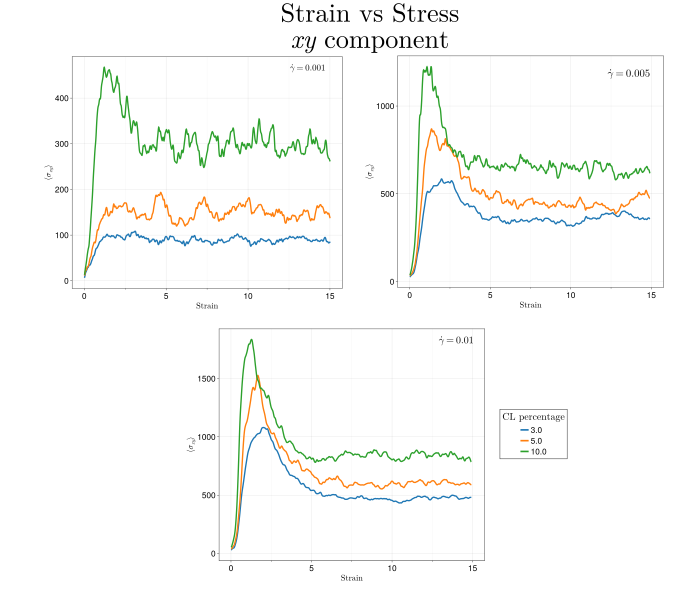
\includegraphics[width=0.9\textwidth]{figs/ComputaitonalResults/zoom-clResponse.pdf}
    \caption{Computational results at different crosslinker concentrations with different shear rates. Each line reprensent the average of 5 experiments with \num{8000} patchy particles with a packing fraction of \num{0.5}, damp of \num{0.5} and the time average is in intervals of \num{5d-2}$\dot{\gamma}$.}\label{fig:stress-strainCLResults}
\end{figure}

Another intriguing finding is the change in the steady-stress regime after the overshoot.
Figure~\ref{fig:yieldStressResults} illustrates the average stress throughout the strain from \num{10} to \num{15} ($\gamma\in[10,15]$) with respect to the shear rate at various crosslinker concentrations.
The dashed lines represent a powerlaw fits $p_1\dot{\gamma}^{p_2}$, where $p_1$ and $p_2$ stands for parameter one and parameter two.
With exponents ($p_2$) $\{0.5901,0.4880,0.4045\}$ for the \num{10}\%, \num{5}\%, and \num{3}\% crosslinker concentrations, respectively.
This finding served as a starting point for further investigation into yield stress events in polymeric networks.
The Herschel-Bulkey model can quantitatively describe a ''\textit{yield stress material},'' and the high congruence between the exponential fit and the numerical results indicates that the polymeric network exhibits similar phenomena.
However, the yield stress $\sigma_y$ was not defined using the Tresca or Von Mises criterion.
Instead, it was chosen to compute the temporal average of the final portion of the deformation, assuming that the system achieves plastic deformation after the overshoot.

\begin{figure}[ht!]
    \centering
    \includegraphics[width=0.9\textwidth]{figs/ComputaitonalResults/yieldStress.pdf}
    \caption{Time average of steady-stress regime from computational results. Dashed lines represent exponential fits.}\label{fig:yieldStressResults}
\end{figure}

%\subsection{Network analysis}

\begin{comment}
In order to describe the network with a quantitative framework, on figure~\ref{fig:network2} we show a set of histograms of the metrics from the gyration tensor for the same system of figure~\ref{fig:network1} along the hole deformation at different shear rates.
This gyration tensor corresponds to the biggest cluster in the simulation.
In panel a it is show the radii of gyration $R_g$, which is the distance of the patchy particle from its center of mass;
in panel b is the shape anisotropy $k^2$, which is \num{0} when all particles are spherically symmetric and \num{1} when all points lie on a line;
in panel c is the asphericity $b$, which has value of zero when the distribution of particles si spherically symmetric or whenever the particle distribution is symmetric with respecto the three coordinate axes, for example any platonic solid;
finally, in panel d is the acylindricity, which is zero when the distribution of particles is cylindrically symmetric or whenever the particle distribution is symmetric with respect to the two coordinate exis, for example, when particles are distributed uniformly on a regular prism.

In general terms, we can see that the increment of crosslinker concentration, the distirbution shifts to the right in the four metrics.
For panels c and d, this means that the cluster starts to deviate from spherical and cylindrical symmetry, meanwhile, for the anisitrpopy parameter, it tells us, that the cluster starts to align into a thin line.
Another important result, is that when the concentration of crosslinker it is increase, the radii of gyration has a more probability to have numeric value around \num{0}, indicating that the morphology of the cluster is spherically symmetric.
\end{comment}

%\begin{figure}[ht!]
%    \centering
%    \includegraphics[width=0.9\textwidth]{figs/ComputaitonalResults/metricsGyrationTensor.pdf}
%    \caption{Gyration tensor metrics for three different shear rates at constant \num{10}\% crosslinker concentration.}\label{fig:network2}
%\end{figure}





